
% Szkielet dla pracy inżynierskiej pisanej w języku polskim.

\documentclass[polish,bachelor,a4paper,oneside]{ppfcmthesis}

\usepackage{polski}
\usepackage[utf8]{inputenc}
\usepackage[OT4]{fontenc}
\usepackage[sectionbib]{chapterbib}

% Authors of the thesis here. Separate them with \and
\author{%
   Krzysztof~Marciniak \album{106574} \and 
   Piotr~Przybysz \album{106602} \and 
   Mikołaj~Szychowiak \album{106580} \and 
   Ryszard~Wojtkowiak \album{106609}}
\title{Projekt i implementacja gry komputerowej z~wykorzystaniem technologii Microsoft~DirectX~11}                   % Note how we protect the final title phrase from breaking
\ppsupervisor{dr~inż.Witold Andrzejewski} % Your supervisor comes here.
\ppyear{2015}                                         % Year of final submission (not graduation!)


\begin{document}

% Front matter starts here
\frontmatter\pagestyle{empty}%
\maketitle\cleardoublepage%

% Blank info page for "karta dyplomowa"
\thispagestyle{empty}\vspace*{\fill}%
\begin{center}Tutaj przychodzi karta pracy dyplomowej;\\oryginał wstawiamy do wersji dla archiwum PP, w pozostałych kopiach wstawiamy ksero.\end{center}%
\vfill\cleardoublepage%

% Table of contents.
\pagenumbering{Roman}\pagestyle{ppfcmthesis}%
\tableofcontents* \cleardoublepage%

\newcommand*{\captionsource}[2]{%
  \caption[{#1}]{%
    #1%
    \\\hspace{\linewidth}%
    \textsc{Źródło:} #2%
  }%
}

% Main content of your thesis starts here.
\mainmatter%

\chapter{Wst\k{e}p}

\section{Cel i~zakres pracy}

Celem pracy jest zaprojektowanie oraz zaimplementowanie gry komputerowej dla systemu Microsoft Windows, przy wykorzystaniu technologii Microsoft DirectX~11. W~ramach niniejszej pracy należy przygotować środowisko, głównie silnik graficzny, wykorzystujący wspomnianą wcześniej technologię. Przedmiotem pracy nie jest implementacja silnika graficznego, możliwe jest więc wykorzystanie istniejących. Narzędzia te mają różne charakterystyki i~nie każde dostępne na rynku będzie przydatne. Dlatego ważny jest wybór odpowiedniego narzędzia. 

Wszelkie informacje na temat  powstawania i~założeń projektu powinny być zapisane w~domumentacji. Stworzenie gry komputerowej wymaga również stworzenia modeli i~animacji. Aby umożliwić rozgrywkę konieczne jest również stworzenie skryptów opisujących mechanikę gry.  

Podczas prac ważna jest praca zespołowa. Tworzenie złożonego projektu od podstaw jest bardzo ważne dla inżyniera, stąd ważne jest wykorzystanie procesów projektowania i~wytwarzania oprogramowania w ramach ninejszej pracy. Procesy te są czasochłonne. Istotne jest więc wykorzystanie metod zarządzania projektami w~celu minimalizacji ryzyka stworzenia wadliwego oprogramowania i~odpowiedniego zarządzania czasem, które pozwoli uniknąć zbędnych opóźnień. 

%Sprawdzić gdzie to ma byc, kto co robił i czy tak może być ujęte
W~ramach niniejszej pracy Krzysztof Marciniak wykonał projekt silnika graficznego, modele 3D i~animacje. 
Piotr Przybysz zaprojektował poziom do gry i~wykonał interfejs użytkownika. 
Mikołaj Szychowiak był odpowiedzialny za zarządzanie projektem oraz rozpoznanie możliwości i~sposobów wykonania wymagań funkcjonalnych.
Ryszard Wojtkowiak zaprojektował broń i~stworzył skrypty mechaniki gry.
Wszyscy członkowie zespołu byli tak samo zaangażowani w~projektowanie oraz testowanie gry.

\chapter{Przegląd zagadnień teoretycznych}

\section{Zarys działania Microsoft DirectX API}

\subsection{Struktura i podstawowe pojęcia}

Microsoft DirectX to interfejs programistyczny (API, ang. \emph{application programming interface}) do tworzenia aplikacji multimedialnych. Składają się na nie przede wszystkim:

\begin{itemize}
\item DirectDraw, Direct2D/Direct3D (komponenty odpowiedzialne za rysowanie grafiki),
\item DirectSound, DirectMusic (obsługa dźwięków),
\item DirectInput (obsługa wejścia - myszy, klawiatury, kontrolerów itp.).
\end{itemize}

DirectX pozwala na tworzenie aplikacji w trzech językach - C\#, Visual Basic oraz C++, przy czym w praktyce spotyka się głównie aplikacje stworzone w C\# oraz C++.
Jak widać na rysunku \ref{directx_infrastructure}, struktura DirectX jest wielopoziomowa i, poza odwołaniami do API oraz komponentami jak na przykład Direct3D 11 (D3D11), obejmuje także DXGI (Infrastruktura Graficzna DirectX, ang. \emph{Microsoft DirectX Graphics Infrastructure}), które -- jako najniższa warstwa -- komunikuje się bezpośrednio ze sterownikiem znajdującym się w przestrzeni jądra systemu operacyjnego. Wykorzystanie komponentów COM (ang. \emph{Component Object Model}) pozwala na łatwą rozbudowę oraz jasny podział funkcjonalności.\\
\begin{figure}
\begin{center}
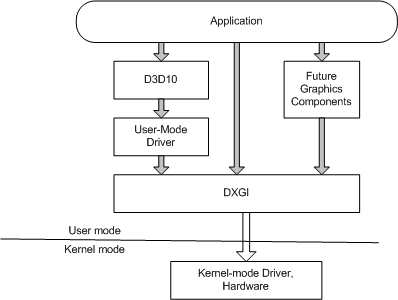
\includegraphics[scale=0.4]{figures/directx_infrastructure.png}
\caption{Architektura DirectX}
\label{directx_infrastructure}
\end{center}
\end{figure}
Podstawowymi i koniecznymi do zrozumienia działania DirectX są koncepcje urządzenia (ang. \emph{device}) oraz jego kontekstu (ang. \emph{device context}).\\
Urządzenie, reprezentowane w wersji 11. przez interfejs ID3D11Device, reprezentuje kartę graficzną i może służyć do tworzenia zasobów oraz pobierania informacji o jej możliwościach (ang. \emph{capabilities}), tj. oferowanych przez nią funkcjonalnościach takich jak np. obsługa podwójnej precyzji w programach cieniujących.\\
Kontekst urządzenia z kolei, jak wskazuje nazwa, określa kontekst użycia urządzenia, co jednoznacznie pokazuje, iż do prawidłowej pracy z urządzeniem powiązany powinien być co najmniej jeden kontekst. Pozwala on głównie na ustawienie stanu w procesie renderingu oraz ustawienie prawidłowych komend wykorzystujących zasoby karty graficznej do wygenerowania obrazu (bezpośrednio na ekran lub do pośredniczącej tekstury, która może zostać wykorzystana później). Wyróżniamy dwa rodzaje kontekstów: bezpośredni/zwykły (\emph{forward}) oraz opóźniony (\emph{deferred}). Bezpośredni wykonuje komendy od razu gdy zostają wywołane, podczas gdy opóźniony pozwala na zapisanie ich na odpowiedniej liście, dzięki czemu mogą zostać wykonane później (jest to przydatne zwłaszcza w przypadku aplikacji wielowątkowych).\\

\subsection{Proces renderingu}

Przebieg wygenerowania grafiki (renderingu) opisywany przez tzw. \emph{pipeline} jest złożony z wielu etapów (ang. \emph{stage}), z których część może być konfigurowana jedynie przez wywołanie odpowiednich komend API poprzedzonych prefiksem będącym skrótem nazwy danego etapu (np. \emph{IA} dla etapu \emph{Input-Assembler}), a część opisywana jest przez programy cieniujące (ang. \emph{shader}).\\
W pipeline DirectX 11 wyróżnia się następujące etapy:
\begin{itemize}
\item Input-Assembler - odpowiada za wczytanie wierzchołków w sposób opisany przez prymityw (trójkąt, czworokąt itp.),
\item Vertex Shader - cieniowanie wierzchołków, ustalanie dla nich wartości początkowych zmiennych jak np. kolor, wektor normalny itp. ,
\item Hull Shader - pierwszy etap teselacji (zagęszczania siatki), przygotowuje siatkę do zagęszczenia przez ustalenie punktów kontrolnych,
\item Tessellator - zagęszcza siatkę wprowadzając dodatkowe prymitywy zastępujące podstawowy i zwraca nowe współrzędne teksturowania,
\item Domain Shader - generuje nowe pozycje wierzchołków na podstawie dwóch poprzednich etapów,
\item Geometry Shader - pozwala zastąpić prymityw wejściowy innym prymitywem,
\item Rasterizer - odpowiada za "spłaszczenie" obrazu tak, aby mógł zostać wyświetlony na ekranie,
\item Pixel Shader - pozwala zmieniać kolor piksela w wynikowym obrazie,
\item Output Merger - generuje końcowy obraz łącząc w odpowiedni sposób (opisany przez komendy takie jak np. OMSetRenderTargets) informacje z poprzedniego etapu.
\end{itemize}

Wszystkie te etapy przedstawione zostały na Rys. \ref{directx_pipeline}. Strzałki określają czy dany etap korzysta jedynie z odczytu danych z karty, czy też pozwala na ich zapis (lub oba równocześnie).

\begin{figure}
\begin{center}
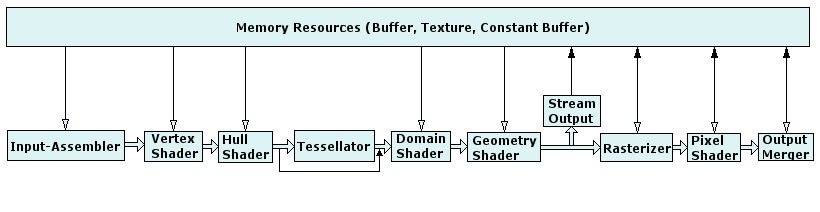
\includegraphics[scale=0.5]{figures/directx_pipeline.png}
\caption{Proces generowania obrazu w DirectX}
\label{directx_pipeline}
\end{center}
\end{figure}

Ostatnim zasługującym na uwagę jest fakt, iż w większości aplikacji wraz z DirectX wykorzystywana jest technologia WinAPI pozwalająca na tworzenie aplikacji graficznych pod platformę Windows. Głównym jej mechanizmem jest pętla komunikatów, których odebranie warunkuje sposób przetwarzania informacji w aplikacji (np. wciśnięcie klawisza powoduje przesunięcie modelu). Komunikaty mogą zostać odczytane w sposób blokujący (przez funkcję \emph{GetMessage}) lub nieblokujący (\emph{PeekMessage}). Z oczywistych względów (tj. narzutu czasowego), w aplikacjach generujących obraz w czasie rzeczywistym wykorzystywana jest wyłącznie funkcja nieblokująca.

\section{Deferred Shading}

Podstawowym sposobem obliczania oświetlenia, uwzględniając opisany wcześniej proces generacji obrazu, jest wyliczenie oświetlenia bezpośrednio dla każdego obiektu. Wartości takie jak wektory normalne, współrzędne teksturowania i inne używane we wspomnianym procesie są wczytywane w shaderze wierzchołków, a następnie interpolowane we fragment/pixel shaderze. W przypadku wielu źródeł oświetlenia (na przykład 200 lub więcej), dla każdego obiektu (niezależnie od tego, czy jest widoczny) należy sprawdzić wszystkie źródła światła, co oznacza złożoność
\begin{equation}
\label{forward_shading_complexity}
O(~liczba\_pikseli\_per\_obiekt~*~liczba\_zrodel\_swiatla~)
\end{equation}
co z kolei w wielu przypadkach jest nie do zaakceptowania (z \ref{forward_shading_complexity} wynika, iż zwiększanie liczby obiektów zmniejsza liczbę źródeł światła, które możemy użyć).\\
Jeśli jednak proces obliczania oświetlania przesuniemy do oddzielnego etapu następującego po wyliczeniu tego, które obiekty są aktualnie widoczne, otrzymamy złożoność
\begin{equation}
\label{deferred_shading_complexity}
O(~liczba\_pikseli~*~liczba\_zrodel\_swiatla~)
\end{equation}
Jak widać z \ref{deferred_shading_complexity}, podejście to nie wprowadza już zależności między liczbą obiektów a liczbą źródeł światła. Pozwala to uzyskać o wiele lepszą wydajność w przypadku scen z wieloma złożonymi obiektami oraz złożonym oświetleniem. Możliwe jest również wprowadzenie wielu uprawnień, jak na przykład podział obrazu na wiele "kafelek" (ang. \emph{tile}), z których każda może zostać obliczona przez wątki na karcie graficznej - technika ta nosi nazwę \emph{tiled deferred rendering} i jest powszechnie stosowana w popularnych silnikach graficznych.\\
Uzyskanie tego efektu wymaga utworzenia kilku tekstur pośredniczących, które łącznie mają nazwę \emph{G-Buffera}. Jest on wykorzystywany do przetrzymywania efektów pośrednich procesu renderingu oraz wyliczenia obrazu końcowego. Format G-Buffera zmienia się w zależności od zastosowania oraz algorytmu obliczania oświetlenia i osoby odpowiadającej za jego implementację, jednak najczęściej wykorzystywane są tekstury:
\begin{itemize}
\item wektorów normalnych,
\item koloru/albedo,
\item głębokości.
\end{itemize}
Pomimo wielu zalet, deferred shading ma jednak swoje wady. Obliczanie oświetlenia z gotowego obrazu uniemożliwia łatwe obliczenie kolorów w przypadku przezroczystych obiektów, zaś wyświetlanie obrazu końcowego w postaci tekstury wymaga wykorzystania bardziej skomplikowanych algorytmów obliczania antyaliasingu, co z kolei obciąża kartę graficzną. Mimo to deferred shading, w zmodyfikowanych odmianach, jest powszechnie wykorzystywany w wielu popularnych grach komputerowych oraz innych aplikacjach renderujących obraz w czasie rzeczywistym.

\section{Podpowierzchniowe Rozproszenie Światła (Subsurface Scattering)}

\section{Depth of Field}


\chapter{Przegląd narzędzi}
Jedną z~najważniejszych kwestii podczas tworzenia gry komputerowej jest prawidłowy dobór narzędzi, ponieważ decyduje to nie tylko o~komforcie pracy, ale także o~jakości końcowego produktu. Podczas tego procesu szczególny nacisk powinien zostać położony na doborze silnika graficznego, między innymi ze względu na dużą dywersyfikację narzędzi należących do tej kategorii oraz mnogość funkcjonalności przez nie oferowanych.

Ze względu na specyfikę tego rozdziału, w~kolejnych punktach opisane zostaną przetestowane rozwiązania wraz z~krótkim podsumowaniem w~formie listy jego zalet i wad. Warto w~tym miejscu również wspomnieć, iż wszystkie analizowane narzędzia oferują możliwość wykorzystania DirectX~11 API, choć niekoniecznie bezpośrednio.

\section{Własny silnik graficzny w~języku C++}
Proces doboru narzędzi rozpoczęto od zaprojektowania i~stworzenia własnego silnika graficznego w~języku C++ w~wersji 11 z wykorzystaniem środowiska Microsoft Visual Studio 2012 na platformę Windows. Pozwoliło to nie tylko na praktyczne wykorzystanie umiejętności nabytych podczas uczestnictwa w zajęciach z Inżynierii Oprogramowania, ale także poznać w praktyce wykorzystanie Microsoft DirectX API w~wersji 11 na najniższym dostępnym poziomie. Tworzenie tego rodzaju oprogramowania wymaga jednak nie tylko odpowiedniej ilości czasu, ale także dobrego zaprojektowania interakcji między klasami oraz zrozumienia wielu zagadnień z~zakresu grafiki komputerowej, w~większości takich, które wykraczają poza program przedmiotu Grafika Komputerowa i Wizualizacja.
Pomimo iż stworzenie własnego silnika oferuje największą swobodę w tworzeniu gry, to podejście okazało się zbyt pracochłonne, aby można je było wykorzystać do realizacji zadanego tematu pracy inżynierskiej w~dostępnym czasie. Na czasochłonność miała wpływ m.in. złożoność tworzonego oprogramowania oraz konieczność wdrażania się członków zespołu w~stworzony przez siebie nawzajem kod.\\

{\raggedright Zalety:
\begin{itemize}
\item większe możliwości w~zakresie wykorzystania DirectX API,
\item lepsza znajomość możliwości oferowanych przez oprogramowanie,
\item brak kosztów.
\end{itemize}

Wady:
\begin{itemize}
\item czasochłonność,
\item wysoki próg wejścia (znajomość m.in. C++ oraz DirectX API),
\item konieczność wytworzenia edytora poziomów i dodatnia odpowiednich funkcjonalności.
\end{itemize}
}
\section{Unreal Engine 4}
Unreal Engine 4 (UE4) jest jednym z~najpopularniejszych silników graficznych dostępnych na rynku, co jest złożeniem wielu czynników. Pierwszym z~nich jest z~pewnością niska cena płatnej licencji (subskrypcja miesięczna to koszt 19\$) oraz darmowy dostęp dla studentów zarówno w~ramach licencji edukacyjnej (należy w~tym wypadku zgłosić chęć wydania licencji w~ramach przedmiotu prowadzonego na uczelni) jak i~w~ramach GitHub Developers Pack (należy jedynie potwierdzić studencki adres e-mail oraz wykorzystać [ang. \emph{redeem}] licencję dostępną na odpowiedniej podstronie serwisu GitHub w~formie kodu [ang. \emph{serial code}]). Drugim jest jakość generowanych (renderowanych) obrazów -- wykorzystanie algorytmu Light Propagation Volumes (algorytm rozwiązywania zagadnienia globalnego oświetlenia w czasie rzeczywistym) pozwala uzyskać niemal fotorealistyczną grafikę, jednak kosztem wysokich wymagań sprzętowych.
Unreal Engine, zarówno w~wersji~3 jak i~4, oferuje dostęp do kodu źródłowego w~języku C++, co - po poznaniu API udostępnianego przez twórców - pozwala szybko i wygodnie rozwijać logikę gry. Umiejętność programowania nie jest jednak wymagana do tego ze względu na obecność mechanizmu blueprintów, który pozwala tworzyć kod z wykorzystaniem bloków oferowanych bezpośrednio w~silniku graficznym.
Ze względu na wysokie wymagania sprzętowe (brak możliwości uruchomienia na komputerach laboratoryjnych oraz komputerach 75\% zespołu) ostatecznie odrzucono to rozwiązanie.\\

{\raggedright Zalety:
\begin{itemize}
\item tania (darmowa) licencja,
\item wygodny edytor i~dostęp do API w~języku C++,
\item niemal fotorealistyczna grafika.
\end{itemize}

Wady:
\begin{itemize}
\item konieczność poznania API,
\item wysokie wymagania sprzętowe.
\end{itemize}
}
\section{Unity}

Unity Engine to obecnie najpopularniejszy silnik graficzny wśród twórców gier niezależnych. Poza płatną licencją oferuje także licencję darmową z okrojoną listą funkcjonalności, które jednak nadal pozwalają na tworzenie dość zaawansowanych gier (wycięte funkcjonalności związane są głównie z jakością grafiki). Ma on także niski próg wejścia ze względu na zastosowanie w skryptach języka C\# lub JavaScript oraz oferuje 30-dniową wersję próbną. Odrzucono go głównie ze względu na wysoką cenę wersji Pro oraz brak pewnych istotnych funkcjonalności (brak miękkich cieni, brak cieni dla źródeł światła innych niż punktowe itp.)\\

{\raggedright Zalety:
\begin{itemize}
\item darmowa (choć okrojona) wersja,
\item niski próg wejścia,
\item 30-dniowa wersja próbna.
\end{itemize}

Wady:
\begin{itemize}
\item gorsza wydajność w stosunku do innych silników (języki C\# i JavaScript oraz wykorzystanie dynamicznych komponentów w trakcie działania powodują powstanie dodatkowego narzutu czasowego),
\item wysoka cena licencji Pro (1500\$),
\item brak pewnych istotnych dla jakości funkcjonalności.
\end{itemize}
}
\section{OGRE}

Object-Oriented Graphics Rendering Engine to elastyczny silnik graficzny o~otwartym kodzie źródłowym napisany w~języku C++. Pozwala na korzystanie z~dwóch API: OpenGL oraz Microsoft DirectX, w tym DirectX 11, przez co został wybrany jako alternatywa dla DirectX 11. Niestety nie jest on rozwijany na bieżąco, przez co wsparcie dla DirectX 11 jest jedynie częściowe i~w~większości wypadków iluzoryczne, ponieważ próba stworzenia urządzenia kończy się rzuceniem wyjątku wewnątrz biblioteki. Nie posiada on także edytora, co znacząco utrudnia tworzenie gier i~ogranicza jego zastosowania do tworzenia dem technologicznych i~testowania nowych technik usprawniających rendering. Ze względu na wspomniane problemy z~obsługą DirectX 11 został on odrzucony po~licznych próbach uruchomienia własnej aplikacji.\\

{\raggedright Zalety:
\begin{itemize}
\item bezpośredni dostęp do DirectX API (otwarty kod źródłowy silnika),
\item (teoretyczne) wsparcie dla DirectX 11.
\end{itemize}

Wady:
\begin{itemize}
\item brak edytora,
\item problemy ze wsparciem dla DirectX 11,
\item kolejne wersje dystrybuowane są wyjątkowo rzadko (ostatnia wersja sprzed dwóch lat).
\end{itemize}
}
\section{CryEngine 3 SDK}

CryEngine 3 Software Development Kit to środowisko stworzone przez firmę Crytek na potrzeby gry \emph{Crysis 3}, a~następnie udostępnione na darmowej licencji. Składa się ono z~edytora oraz kodu źródłowego w~języku C++ wraz z~projektem środowiska Microsoft Visual Studio. Dostęp do kodu źródłowego pozwala na lepszą kontrolę nad tworzoną aplikacją, jednak ogranicza się to głównie do mechaniki rozgrywki, ponieważ system renderujący został udostępniony jako biblioteka dołączana do~projektu. Kolejnym mankamentem tego rozwiązania jest brak dokumentacji dla wielu funkcji, metod oraz opcji edytora, w~tym dla rozproszenia podpowierzchniowego, które jest jedyną oferowaną funkcjonalnością DirectX 11. Edytor nie pozwala też na tworzenie programów cieniujących, co mogłoby pozwolić na stworzenie własnych rozwiązań problemów (na przykład wspomniane przybliżone rozwiązanie z~mapą głębokości). Ze względu na wymienione trudności z~rozwojem projektu w~tym środowisku ostatecznie zostało ono odrzucone.\\

{\raggedright Zalety:
\begin{itemize}
\item dostęp do kodu źródłowego silnika,
\item wsparcie dla DirectX 11,
\item łatwy w obsłudze edytor.
\end{itemize}

Wady:
\begin{itemize}
\item ograniczone możliwości,
\item brak możliwości tworzenia własnych programów cieniujących,
\item niekompletna dokumentacja.
\end{itemize}
}

\section{Unreal Engine 3}

\section{Unreal Development Kit (UDK)}

\section{Autodesk Maya}

\section{Autodesk 3D Studio Max}

\section{Blender}

\section{Gimp}

Do tworzenia menu a także szablonu poziomu wykorzystano oprogramowanie o nazwie Gimp. Istotną jego zaletą jest to, że jest to darmowy a oferujący sporo możliwości program. Dodatkowo obsługa Gimpa jest prosta, dzięki czemu szybko stworzone potrzebne grafiki.

\section{Adobe Flash - Scaleform}

Każda gra powinna mieć menu główne. W celu jego stworzenia wykorzystano wtyczkę do Adobe Flash Professional o nazwie Scaleform. Wtyczka ta służy do tworzenia interfejsów graficznych występujących na przykład w grach. Wykorzystano to, że darmowa jej wersja jest zawarta w UDK. Do jej zainstalowania potrzeba było pobrać Adobe Flash Professional a także Adobe Extension Managera. Problemem było rozszerzenie wtyczki. Było ono kompatybilne tylko ze starymi wersjami Adobe Flash Professional, a te niestety nie działały na Windowsie 8.1. W związku z tym konieczne stało się dodatkowe pobranie 
Adobe Extension Managera CS6 i przekonwertowanie wtyczki ze Scaleformem z rozszerzenia mxp na zxp.
Po przekonwertowaniu nowa wersja działała z Adobe Flash Professional CC, który wykorzystano w projekcie. Sam Scaleform jest prosty w obsłudze i intuicyjny, wykorzystuje flasha, a dodatkowo jest kompatybilny z UDK i łatwo można za jego pomocą połączyć menu z grą.

{\raggedright Zalety:
\begin{itemize}
\item łatwość obsługi,
\item cena (darmowa wtyczka, zawarta w UDK),
\item kompatybilność z UDK.
\end{itemize}

\raggedright Wady:
\begin{itemize}
\item konieczność przekonwertowania wtyczki,
\item problemy z instalacją,
\item konieczność instalacji dodatkowego oprogramowania.
\end{itemize}
}

\section{Git}

W projektach nad którymi pracuje kilka osób niemożliwa jest praca bez systemu kontroli wersji. Początkowo, ze względu na pracę z kodem źródłowym, skorzystano z systemu Git ze względu na łatwość użycia oraz możliwość utworzenia prywatnego repozytorium na koncie studenckim w serwisie GitHub. Niestety ze względu na przejście na Unreal Development Kit konieczne było skorzystanie z narzędzia Perforce.\\

\raggedright Zalety:
\begin{itemize}
\item łatwość obsługi,
\item dobra obsługa plików tekstowych,
\item prywatne repozytorium w serwisie GitHub dla studentów.
\end{itemize}

\raggedright Wady:
\begin{itemize}
\item problemy z obsługą dużych plików binarnych,
\item brak integracji z Unreal Development Kit.
\end{itemize}

\section{Perforce}

Ostatnim opisywanym narzędziem jest system kontroli wersji Perforce, który dobrze obsługuje duże pliki binarne, dzięki czemu jest popularny w firmach zajmujących się wytwarzaniem oprogramowania (w tym gier). Pozwala on również -- w przeciwieństwie do gita -- na integrację z edytorem Unreal Development Kit, co znacząco przyspiesza i ułatwia pracę. Niestety ma on również swoje wady, które ujawniają się dopiero z upływem czasu, na przykład problemy z obsługą usuniętych plików (nadal uwzględniane są w listach zmian) czy nie zapisywanie zmian wprowadzonych w plikach na wspomniane listy.

\raggedright Zalety:
\begin{itemize}
\item dobra obsługa plików binarnych,
\item integracja z Unreal Development Kit.
\end{itemize}

\raggedright Wady:
\begin{itemize}
\item niespodziewane problemy wynikające z niewłaściwej obsługi zmian,
\item konieczność zainstalowania dedykowanego oprogramowania serwerowego i utrzymania serwera.
\end{itemize}

\section{Jira}

Przy pracy w kilkuosobowych zespołach przydaje się również oprogramowanie do zarządzania projektem. Skorzystano tu z platformy Jira. Umożliwia ona przydział zadań do poszczególnych członków zespołu. Ułatwia to pracę w wiele osób, poniewż zabezpiecza przed sytuacją, w~której kilka osób będzie wykonywało to samo zadanie. Wbudowany system szacowania czasu realizacji zadania pomaga oszacować czas potrzebny na stworzenie danej funkcjonalności i~zakończenie projektu. Jira posiada również możliwość zintegrowania z systemem kontroli wersji, co pozwala śledzić postęp prac, na podstawie komentarzy przy tworzeniu kolejnych rewizji.

Zalety:
\begin{itemize}
\item możliwość estymowania czasu wykonywania zadania
\item integracja z systemami kontroli wersji
\item duża liczba dodatków
\item definiowanie priorytetów zadań
\end{itemize}

Wady:
\begin{itemize}
\item tylko płatna licencja
\item nie do końca czytelny interfejs
\end{itemize}
\chapter{Praca własna}
Proces twórczy został podzielony na dwa główne etapy: projektowanie i~implementację. Ponieważ tworzenie gry wymaga przygotowania oraz doboru odpowiedniego środowiska, etapy te zostały poprzedzone analizą problemu oraz burzą mózgów na której zarysowały się wstępne wymagania funkcjonalne. Zdefiniowane zostały również główne wymagania pozafunkcjonalne, takie jak docelowa platforma obsługująca grę. W celu zapewnienia spójnej wizji gry wśród członków zespołu, postanowiono skonstruować dokument, zawierający opis wszystkich decyzji podjętych podczas tworzenia projektu oraz wyjaśnienia dotyczące wszystkich wymagań funkcjonalnych oraz pozafunkcjonalnych -- Game Design Document (GDD), stanowiący jednocześnie załącznik~1 do niniejszej pracy.  Pomysły zebrane podczas burzy mózgów zostały poddane wnikliwej analizie, co pozwoliło na stworzenie spójnej wersji projektu. 

\section{Projektowanie}
Projektowanie jest bardzo ważnym etapem prac nad każdym projektem informatycznym. Pozwala uspójnić wizję gry w~zespole oraz zdefiniować zadania, które będą wykonywane podczas implementacji. Dlatego dobrze, gdy na tym etapie pracy w proces twórczy zaangażowany jest każdy członek zespołu. 

Istnieje wiele sposobów na projektowanie gry komputerowej. Podejściem, które ułatwia stworzenie gry, która bawi, jest projektowanie zorientowane na gracza. Zgodnie z~charakterystyką przedstawioną w~\cite{Adams:pgp}, stosując tę metodę, twórcy powinni wyobrazić sobie typowego gracza, a~więc osobę, dla której ta gra jest tworzona. Aby użytkownik był zadowolony, należy zapewnić mu rozrywkę -- jest to podstawowa funkcja gry. W~tym celu należy utożsamić się z~graczem. Pozwoli to wybrać funkcje, które uczynią grę atrakcyjną.

Istotnym elementem tworzenia projektu gry jest wnikliwa analiza wymagań funkcjonalnych oraz uszeregowanie ich według wagi. Każdy z członków zespołu posiadał własną wizję gry. Połączenie ich wszystkich zaowocowało spójnym projektem, opisanym w~załączniku~1 -- GDD. 

Aby zapewnić, że projekt będzie spójny, konieczne jest stworzenie dokumentów projektowych. Powstrzymuje to programistów przed puszczaniem wodzy fantazji i~tworzeniem funkcjonalności niezgodnych z projektem. 

Na tym etapie przydatna okazała się nie tylko teoretyczna wiedza na temat tworzenia zaawansowanych projektów informatycznych, ale przede wszystkim doświadczenia innych twórców gier, które zespół poznał przy okazji udziału w~konferencjach takich jak Zjazd Twórców Gier (ZTG) czy World of Gamedev Knowledge (WGK). Zdobyto wiedzę potrzebną między innymi do stworzenia poziomów ciekawych dla graczy, wyboru funkcjonalności nie wymagających skomplikowanych i~często zawiłych implementacyjnie elementów (co często powoduje błędy i~trudności w~dalszym rozwoju projektu), jednocześnie będących skomplikowanymi z~punktu widzenia gracza. 

Dobrą praktyką przy tworzeniu gry jest również częste testowanie graficznego interfejsu użytkownika, jego czytelności i~łatwości użycia kluczowych funkcji w~ferworze walki. Pozwala to zaprojektować interfejs przyciągający wzrok oraz funkcjonalny. Projektując HUD [ang. \emph{Head-Up Display}], a~więc wszystkie istotne w~trakcie rozgrywki wskaźniki, mapkę, poziom życia; postanowiono rozmieścić interesujące dla graczy informacje analogicznie do popularnych gier z~gatunku strzelanek. Jest to dla nich atrakcyjne, ponieważ nie muszą zmieniać swoich przyzwyczajeń by sprawdzić poziom życia. 

Jednak projektowanie to nie tylko uspójnienie rozgrywki, ale również specyfikacja dotycząca środowiska, w~którym gra powstanie. W tym celu należało wybrać odpowiednie narzędzia, co zostało opisane w~Rozdziale 3: Przegląd narzędzi. 

\subsection{Projekt silnika graficznego}

W ramach pracy jako pierwsze przetestowano podejście z~tworzeniem własnego silnika graficznego w~języku C++. Jak zostało wspomniane w~poprzednim rozdziale, tworzenie tego rodzaju oprogramowania wymaga pewnej określonej wiedzy dotyczącej zarówno architektury silników~graficznych i~inżynierii oprogramowania, jak i~grafiki komputerowej oraz Microsoft DirectX API. Jako że wiedza teoretyczna wraz z podstawowymi pojęciami zostały zarysowane w rozdziale 2., tutaj opisane zostaną kwestie dotyczące architektury silnika oraz usprawnień, które mogłyby zostać wprowadzone w~przyszłości.\\

W silniku graficznym można zasadniczo wydzielić 3 podstawowe składowe:
\begin{itemize}
\item renderer - przeprowadza proces renderingu, tj. generowania grafiki,
\item menedżer obiektów - zawiera listę obiektów i/lub listę ich grup,
\item menedżer zasobów - odpowiada za alokację i zwalnianie zasobów takich jak tekstury, dźwięki itp.
\end{itemize}

W ramach menedżera obiektów zastosowano wzorzec kompozyt ze względu na jego idealne dopasowanie do problemu.
Jak widać każda z~tych składowych może stanowić pewną jednostkę (ang. \emph{entity}) budującą system - w~tym wypadku system graficzny (wyróżnia się również na przykład systemy fizyki). Jednostki można również podzielić na mniejsze komponenty, które można dynamicznie dodawać i~usuwać w trakcie działania - podejście takie zgodne jest wzorcem \emph{Entity-Component-System}. Jak zauważono podczas testowania opisywanego oprogramowania, poza wygodą oraz nowymi możliwościami rozwoju wykorzystanie dynamicznych komponentów wprowadza także narzut czasowy ze względu na wykorzystanie metod wirtualnych oraz nieoptymalne wykorzystanie pamięci podręcznej procesora. W~tym wypadku możliwym usprawnieniem mogłoby być budowanie aplikacji z~komponentów w~edytorze, a~następnie generowanie "stałych" klas i~kompilowanie zmodyfikowanego w~ten sposób kodu do pliku wykonywalnego, który mógłby być dystrybuowany jako gotowa aplikacja.\\
Nieoptymalne wykorzystanie pamięci podręcznej procesora dotyczy nie tylko wykorzystania komponentów, gdyż jest wąskim gardłem większości zarówno amatorskich jak i~profesjonalnych silników graficznych. W~celu zniwelowania tego problemu można utworzyć pewien stały obszar pamięci (w~języku C++ w~wersji 11. w tym celu wykorzystać można operator \emph{placement new}) i~utworzyć pulę obiektów, w~ramach której mogłyby one być używane ponownie bez konieczności zwalniania zajmowanej przez nie pamięci.\\
Ostatnim usprawnieniem, które można byłoby wprowadzić celem zwiększenia efektywności procesu renderingu jest wielowątkowość, która jednak wymagałaby wprowadzenia synchronizacji między wątkami aplikacji (np. zamki) oraz użycia metod DirectX obsługujących wielowątkowość (np. operować na opóźnionym kontekście urządzenia). Jej użycie utrudniałoby też skuteczną naprawę błędów ze względu na brak możliwości odpluskwiania kodu w środowisku Microsoft Visual Studio, w którym tworzone było to oprogramowanie.\\
Dla silnika została napisana i wygenerowana z wykorzystaniem aplikacji Doxygen dokumentacja, jednak ze względu na swoją objętość (150 stron) nie została tutaj załączona.
% dodawać wykaz klas, przestrzeni nazw i kod źródłowy + dokumentację w pdf?
% dodać do literatury tekst o EntityComponentSystem + o deferred shading i tutoriale z animacji

\subsection{Modele 3D i animacje}



\subsection{Projekt poziomu}
Do stworzenia poziomu wykorzystano środowisko Unreal Development Kit (w skrócie UDK), do którego zaimportowano wcześniej stworzone modele. Niewątpliwą zaletą UDK jest możliwość szybkiego stworzenia poziomu poprzez przenoszenie obiektów z panelu edytora prosto na tworzoną mapę. A także oprogramowanie wydarzeń występujących na niej zgodnie z zasadami programowania wizualnego, za pomocą komponentów, układanych obok siebie i łączonych liniami z wykorzystaniem interfejsu graficznego.

W tworzeniu poziomu istotne jest jego umiejscowienie w realiach rozgrywki. Poziom powinien być powiązany z fabułą i światem przedstawionym. W związku z tym istotne było określenie czasu i miejsca akcji. Ponieważ podczas burzy mózgów ustaliliśmy, że fabuła gry będzie polegać na potyczkach żelków to istotne stało się dopasowanie miejsca aby zwiększyć immersję a co za tym idzie przyjemność z gry. W związku z tym, że żelki są jedzeniem a jedzenie jest powiązane z kuchnią, oczywisty stał się wybór tego pomieszczenia jako miejsce starcia. Stworzono, więc wstępny projekt poziomu. Stworzono go w programie Gimp. Jego celem był wstępny zarys, zorientowanie się jak co powinno wyglądać a także przekazanie informacji, jakie tekstury wykonać. Wstępny projekt został stworzony szybko i zawiera jedynie kontury obiektów, gdyż służy głównie do zorientowania się w koniecznych do stworzenia modelach oraz skonsultowania z członkami grupy rozmieszczenia elementów w celu zwiększenia przyjemności z gry, gdyż każdy z nich grał wcześniej w tego typu gry i ma doświadczenie z gry na wielu planszach i może pomóc lepiej zaprojektować poziom. Istotną bowiem sprawą w tworzeniu poziomu jest takie jego zaprojektowanie by był sprawiedliwy i dawał graczom dużo możliwości, różnego poprowadzenia rozgrywki. Dlatego obmyślono stworzenie stołu po którym gracz będzie mógł się wspinać i zaskakiwać przeciwników z wysokości a także porozrzucanie po pomieszczeniu (w tym przypadku kuchni), obiektów służących jako osłony, dzięki czemu łatwiej będzie się schować i zaskoczyć oponenta, tym samym zmniejszając wielkość otwartych przestrzeni, które na podstawie doświadczeń grupy w zbyt dużej liczbie obniżają przyjemność płynącą z grania poprzez zmniejszenie możliwych taktyk.

Następnym krokiem było stworzenie poziomu w edytorze. W tym celu wykorzystano gotowe modele i zaprojektowano mieszkanie 3 pokojowe z korytarzem. Zwiększenie liczby pomieszczeń miało na celu zwiększenie możliwych punktów startu a także oddalenie ich od siebie w celu nie natrafienia od razu na przeciwnika. W innym przypadku mogłoby wyniknąć niezadowolenie z rozgrywki, z powodu różnic komputerów biorących udział w rozgrywce, ładują one poziom w różnym czasie, więc możliwe są drobne różnice czasu. A ponieważ strzelanki to gatunek gier szybkich, nawet niewielka różnica może zadecydować o zwycięstwie w potyczce. Dodatkowo w poziomie uwzględniono możliwość wspinania się (oprócz stołów) na niektóre obiekty, a także wykorzystanie kilku szklanych przeszkód (niezależnie od normalnych przeszkód), przez które widać przeciwnika, a których nie można zniszczyć. Umożliwia to bowiem ukazanie możliwości Directx 11 a także urozmaica rozgrywkę.

Poziom został stworzony z myślą o grze wieloosobowej w trybie każdy na każdego, w związku z tym nie było potrzeby tworzenia specjalnych sektorów dla każdej drużyny, a co za tym idzie jest więcej punktów startowych i w kolejnych rozgrywkach możliwe jest wylosowanie innego, więc konieczne są modyfikacje taktyki i sposobu gry, wynikające z innego otoczenia startowego.

\section{Implementacja}

\subsection{Wykorzystanie technologii DirectX 11 w~UDK}

W ramach wsparcia DirectX 11, Unreal Development Kit obsługuje trzy opisane w~rozdziale teoretycznym techniki: rozproszenie podpowierzchniowe (subsurface scattering), deferred shading (znany także jako \emph{deferred rendering}) oraz rozszerzenie techniki głębi ostrości o~nazwie \emph{bokeh depth of field} (bokeh [od jap. \emph{boke} w romaji - rozmycie] to efekt rozmycia obrazu z pewnym zniekształceniem, którego kształt zależy od kształtu soczewki - Rys. \ref{bokeh_example}).\\

Technikę rozproszenia podpowierzchniowego wykorzystano w~celu stworzenia materiału, z~którego wykonany jest gracz. Zgodnie z~\cite{udk_sss}, aby tego dokonać, należy najpierw aktywować opcję ''Enable Subsurface Scattering'' w~zakładce ''D3D11'', a~następnie ustawić wymagane parametry, czyli kolor światła rozproszonego (SubsurfaceInscatteringColor), kolor światła pochłoniętego (SubsurfaceAbsorptionColor) oraz promień rozproszenia (SubsurfaceScatteringRadius). W celu uzyskania realistycznego wyglądu materiału, zmieniono także metodę mieszania na ''BLEND\_Translucent'' (pozwala to uzyskać materiał półprzezroczysty, w przeciwieństwie do domyślnej wartości BLEND\_Opaque). Na Rys. \ref{sss_material} przedstawiony został widok materiału w edytorze, zaś na Rys. \ref{sss_material_example} - przykłady jego użycia.\\

Z~\cite{udk_bokeh_dof} wynika, iż użycie techniki Bokeh Depth of Field wymaga jedynie utworzenie odpowiedniej tekstury (w~niniejszej pracy użyto tekstury pięciokąta foremnego pokazanej na~Rys. \ref{bokeh_texture}) oraz ustawienia wartości ''DepthOfFieldType'' na ''BokehDOF'' w efekcie końcowym procesu renderingu (etap ten nie ma swojej nazwy w języku polskim, natomiast oryginalnie nosi nazwę \emph{post-processing}).\\

Ostatnia funkcjonalność DirectX 11, czyli Deferred Shading jest włączona domyślnie gdy używany jest renderer DX11, dzięki czemu nie było koniecznym włączenie tej opcji ręcznie.

\begin{figure}
\begin{center}
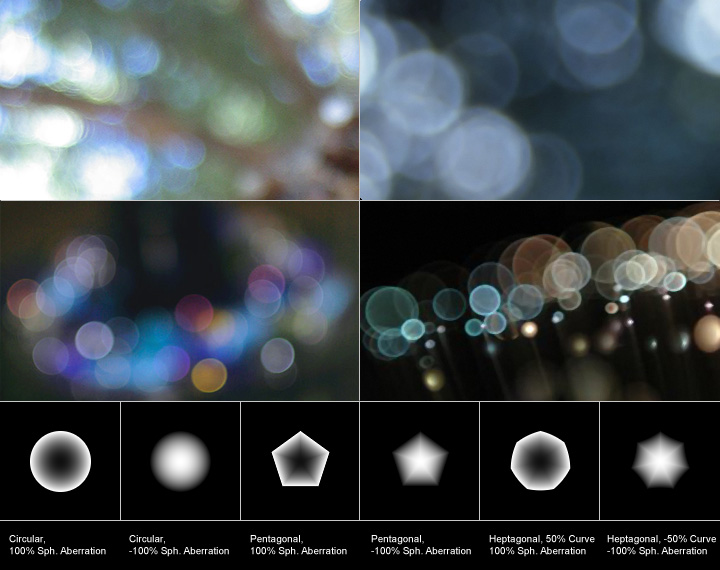
\includegraphics[scale=0.4]{figures/bokeh.jpg}
\captionsource{Rodzaje bokeh}{http:\/\/www.dofpro.com\/gallery\/dofpro\_spherical\_aberrations.jpg}
\label{bokeh_example}
\end{center}
\end{figure}

\begin{figure}
\begin{center}
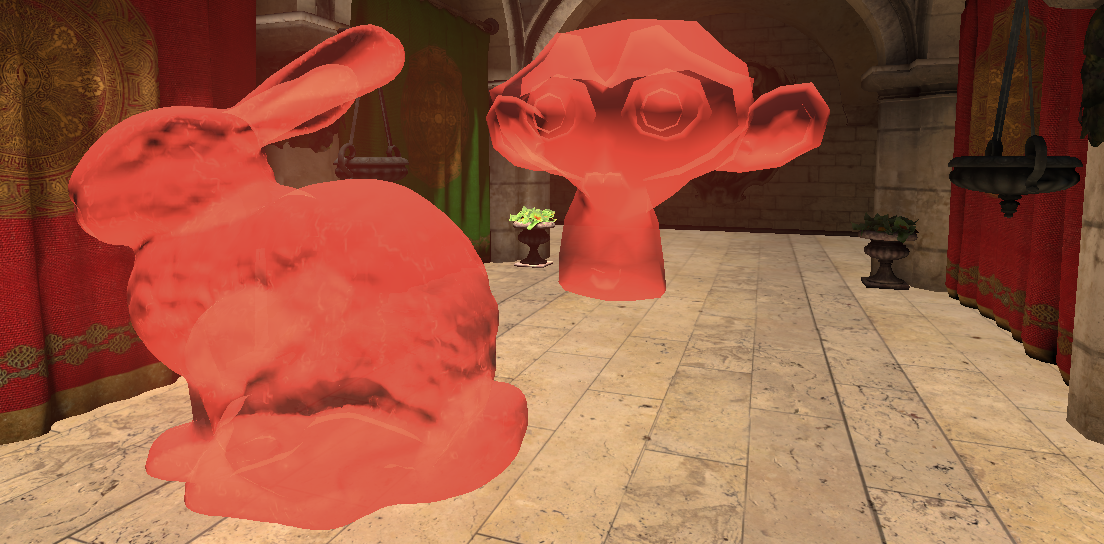
\includegraphics[scale=0.4]{figures/jelly_material.png}
\caption{Przykłady użycia materiału wykorzystującego rozproszenie podpowierzchniowe}
\label{sss_material_example}
\end{center}
\end{figure}

\begin{figure}
\begin{center}
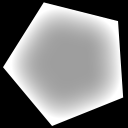
\includegraphics[scale=0.6]{figures/T_Bokeh_Pentagon.png}
\caption{Tekstura bokeh użyta w tworzonej grze}
\label{bokeh_texture}
\end{center}
\end{figure}

\subsection{Zarządzanie projektem}
W~celu sprawnej organizacji pracy w~zespole wykorzystano metody zarządzania projektami. Uspójnienie projektu gry podczas fazy projektowania pozwoliło na zdefiniowanie i~wyspecyfikowanie zadań, realizowanych podczas implementacji. Znając liczbę zadań, można było podzielić projekt na kolejne przyrosty. Projekt miał być realizowany z~wykorzystaniem metod zwinnych. Trudnością w~wykorzystaniu typowej zwinnej metody, takiej jak programowanie ekstremalne czy Scrum okazał się charakter projektu, będącego pracą dyplomową. Z~tego względu narzucony został ostateczny termin ukończenia produktu. Jest to sprzeczne z manifestem zwinności, dlatego zdecydowano się na inne rozwiązanie.

Początkowo użyto modelu kaskadowego. Jego zaletą jest sekwencyjność, pozwalająca oddzielić procesy analizy problemu, projektowania, implementacji oraz testowania i~późniejszego utrzymania projektu, co przedstawiono na Rys. \ref{waterfall}. Metoda Waterfall, wykorzystująca ten model, nie jest jednak pozbawiona wad. Dotyczą one głównie dużych projektów, a~więc nie miały miejsca w~przypadku oprogramowania tworzonego w~czteroosobowym zespole programistów. Korzystając z~tej metody oszczędza się czas na planowaniu. Jak opisano w~\cite{Kaczor:Scrum}, faza ta zajmuje zaledwie 25\% czasu pracy nad projektem. Rezultat końcowy zostaje ustalony jeszcze przed rozpoczęciem implementacji, podobnie jak poszczególne przyrosty implementacji. Każdy przyrost miał trwać 2 tygodnie i~zawierał określone zadania. Rezultatem końcowym był produkt posiadający wartość biznesową, w~tym przypadku - w~pełni działająca gra. Co istotne, wartość biznesową produkt miał zyskać dopiero w~przedostatnim przyroście. 

\begin{figure}
\begin{center}
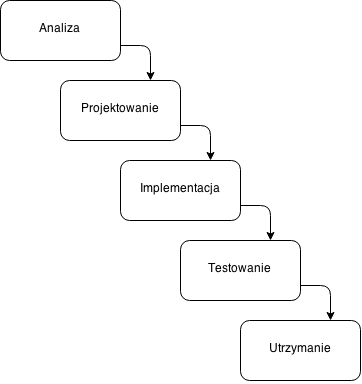
\includegraphics[scale=0.4]{figures/waterfall.png}
\caption{Model kaskadowy}
\label{waterfall}
\end{center}
\end{figure}

Problemem w~wykorzystaniu modelu kaskadowego są błędy, wykryte podczas fazy testowania. Ponieważ w~momencie rozpoczęcia testów cały produkt jest już zaimplementowany, poprawka może spowodować powstanie kolejnych błędów. Może jednak się zdarzyć, że błąd powstał na etapie projektowania, w~takim przypadku należy powtórzyć tę fazę, jak również całą fazę implementacji. Powoduje to wydłużanie czasu realizacji oraz wzrost kosztów wytworzenia produktu.

W~niedługim czasie po zaplanowaniu prac nad projektem okazało się, że metoda ta nie jest wystarczająca, zaczęło się pojawiać opóźnienie w~pracach, które mogło spowodować pogorszenie jakości produktu. Zdecydowano się więc skorzystać z~metod zwinnych. Metodyki Agile charakteryzują się stałą jakością, a~sterowane są zakresem. W~omówionej wcześniej metodzie Waterfall zakres był stały, zmieniała się jedynie jakość, a~chęć utrzymania wysokiej jakości powodowała opóźnienie względem planu. 

Ostatecznie zastosowano metodykę zwinną zbliżoną do metody Feature-Driven Development, wplatając w~nią elementy metodologii Scrum. Zadania podzielono na część dotyczącą rozpoznania danego zagadnienia i~część implementacyjną. 

W~części dotyczącej rozpoznania zastosowano cykl PDCA (\emph{Plan -- Do -- Check -- Act}), stworzony przez Williama Edwardsa Deminga. Pierwszy etap cyklu -- planowanie -- polegało na zapoznaniu się z~opisem wybranej funkcjonalności, zawartym w~Game Design Document. Następnie, w~fazie wykonania, zbierano informacje na temat możliwości implementacji funkcjonalności wykorzystując UDK oraz próbowano stworzyć wybraną funkcję. W~trzeciej fazie sprawdzano czy zaimplementowana wersja funkcji odpowiada założeniom projektu. Jeśli wynik był pozytywny, funkcjonalność została wybierana do wykonania w~kolejnym przyroście.

Realizowane były tygodniowe sprinty (przyrosty). Każdy sprint rozpoczynał się spotkaniem zespołu, na którym omówiono pozostałe zadania oraz zaplanowano jakie funkcjonalności będą implementowane w~kolejnym przyroście. W~efekcie udało się zachować jakość wykonania oraz zakończyć prace przed upływem niezmiennego terminu ukończenia, modyfikując nieznacznie zakres dostępnych funkcjonalności. Zespół tworzący grę był wskroś-funkcjonalny, co oznacza, że członkowie zespołu wykonywali zadania dotyczące różnych zagadnień. Począwszy od tworzenia prostych modeli 3D po skryptowanie. Jest to cecha charakterystyczna metody Scrum. Z~kolei sposób planowania kolejnych przyrostów, a~więc planowanie ze względu na funkcjonalność, zaczerpnięto z~metody Feature-Driven Development. 

Na koniec każdego przyostu otrzymywano prototyp posiadający pewną funkcjonalność. Jeśli funkcjonalność działała prawidłowo podczas testów, dołączano ją do głównego prototypu, który z~każdym przyrostem stawał się bardziej funkcjonalny, aż w~końcu stał się wersją produkcyjną. Ze względu na wcześniejszy nieudany eksperyment z~metodą Waterfall wartość biznesową projekt zyskał dopiero po kliku przyrostach. Oznacza to, że pierwsze efekty nie były satysfakcjonujące, jednak prezentowały postęp prac. 

\begin{figure}
\begin{center}
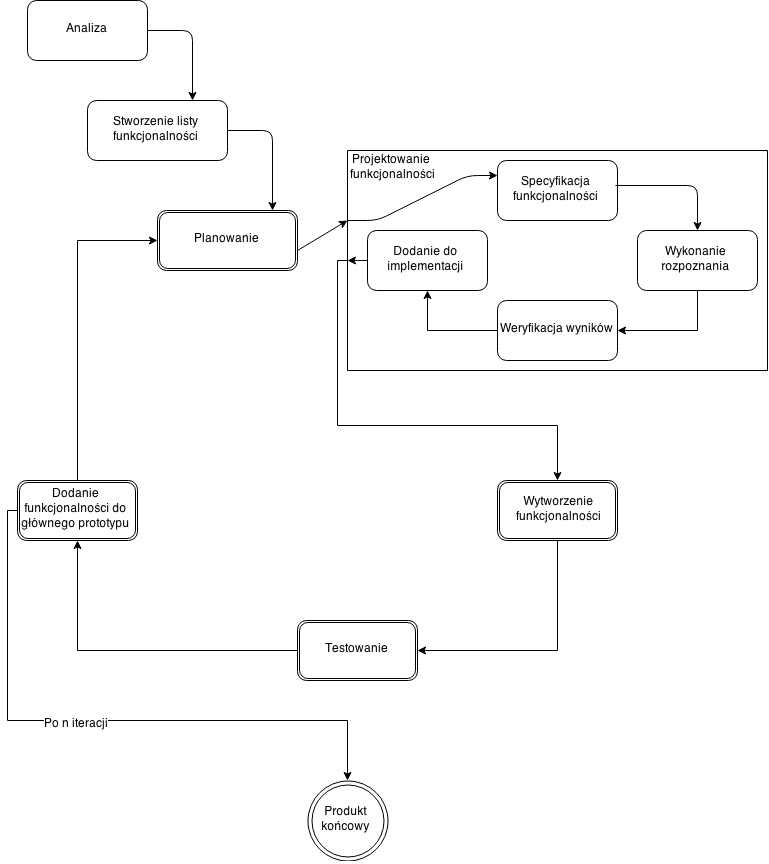
\includegraphics[scale=0.4]{figures/ujelly_phases.png}
\caption{Etapy procesu wytwórczego gry przy wykorzystaniu metody Feature-Driven Development i~cyklu PDCA}
\label{ujelly_phases}
\end{center}
\end{figure}

Trzy główne fazy procesu wytwarzania gry, występujące w~modelu kaskadowym, a~więc: projektowanie, implementacja i~testowanie, w~metodach zwinnych są wykonywane w~każdym sprincie, co znacznie zmniejsza ryzyko powstania krytycznych błędów po zaimplementowaniu całego produktu. W~przypadku wykorzystania Feature-Driven Development proces naprawy błędów również obarczony jest mniejszym ryzykiem czasowym. Zwłaszcza, gdy błąd powstał na etapie projektowania danej funkcjonalności. W~skrajnym przypadku, wadliwa funkcjonalność nie trafi do głównego produktu.

\chapter{Podsumowanie}

Celem pracy inżynierskiej było stworzenie gry komputerowej. Proces ten okazał się długotrwały i wyboisty. Istotne zatem było podzielenie pracy na kilka części, które równomiernie podzielono. Dzięki temu żaden z członków grupy nie nadpisywał pracy innego i każdy mógł działać równolegle. Tworzenie gry wymagało korzystania z technologii i programów nie przerabianych na studiach. Dzięki temu poszerzono swoje horyzonty. Zobaczono jak to jest pracować nad grą w profesjonalnym środowisku którego używają na co dzień firmy produkujące produkcje na masową skalę. Postanowiono stworzyć grę tak jak to robią wielkie firmy, więc stworzono GDD. Wykorzystano również niektóre metodyki zwinnego programowania. Dzięki temu znacznie przyspieszono pracę. Utrapieniem były problemy z konfiguracją i środowiskiem. Wybór odpowiedniego nie był łatwym zadaniem, spowodowało to konieczność przetestowania wielu z nich. Niektóre trzeba było odrzucić z powodu zbyt niskich możliwości sprzętowych. To tylko dowodzi, że trudno tworzyć gry w nowej technologii bez drogiego sprzętu.

Stworzenie własnej gry komputerowej dostarcza wielu cennych porad. Dzięki uczeniu się na własnych błędach i odpowiednim podejściu do pracy, można przyspieszyć ten proces. Na przykład, nie da się znaleźć odpowiedniego środowiska bez licznych testów, dzięki którym wiadome było co jest istotne i czego potrzeba w grze a jakie są granice środowiska graficznego które nas ograniczają, w związku z tym istotny był wybór odpowiedniego, takiego które daje najwięcej możliwości za jak najniższą cenę.
% Bibliography (books, articles) starts here.
\chapter{Literatura}
\renewcommand{\section}[2]{}
\bibliographystyle{plalpha}{\raggedright\sloppy\small\bibliography{bibliography}{}}
%\bibliographystyle{plalpha}{\raggedright\sloppy\small\bibliography{bibliography}}
\chapter{Dodatki}

\appendix
\chapter{Game Design Document}
\label{chap:gdd_appendix}

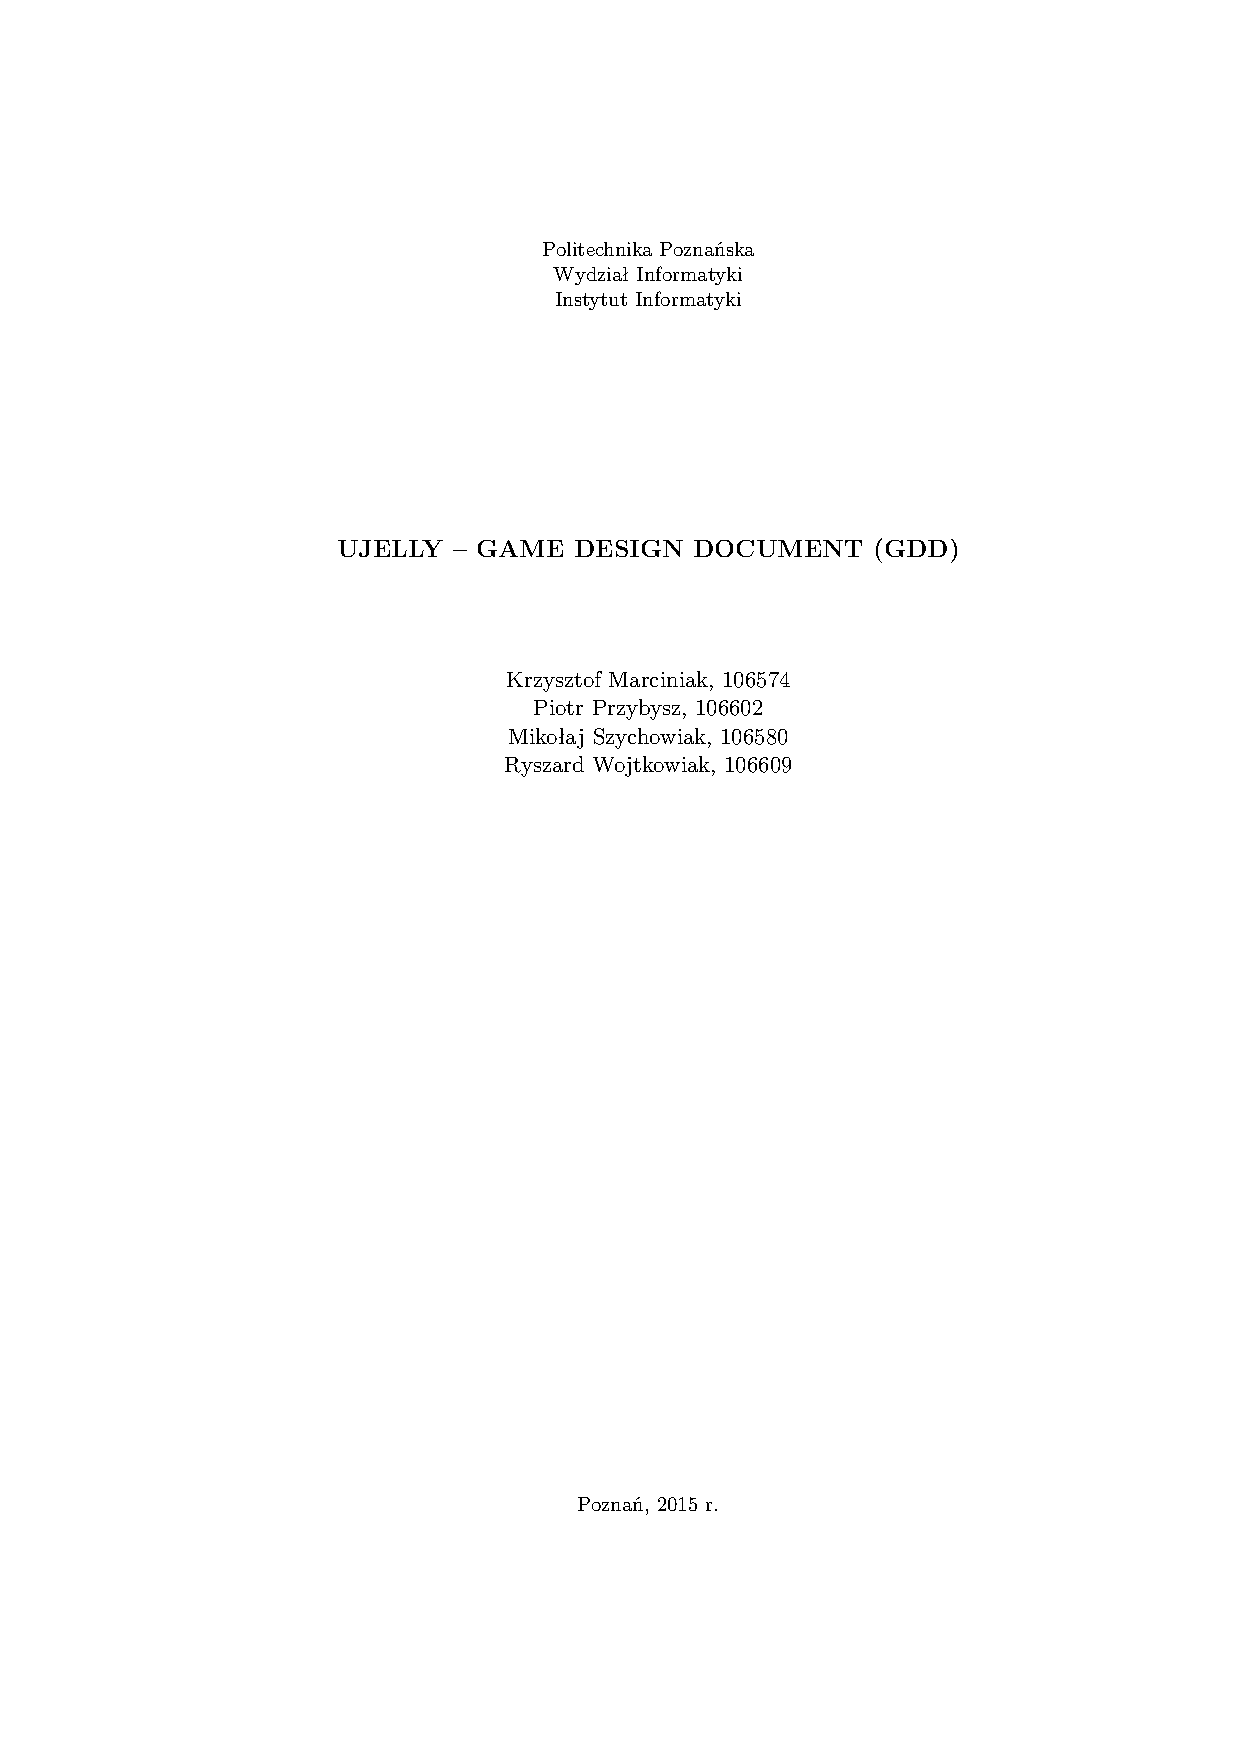
\includepdf[pages={1,3-12}]{game_design_document.pdf}

% All appendices and extra material, if you have any.
\cleardoublepage\appendix%


% Colophon is a place where you should let others know about copyrights etc.
\ppcolophon

\end{document}
